\documentclass[english]{article}

\usepackage[utf8]{inputenc}
\usepackage[T1]{fontenc}                                    % Font encoding
\usepackage{babel}                                          % Translation
\usepackage[babel]{csquotes}                                % Quotes
\usepackage{newtxtext,newtxmath}                            % Times font
\usepackage{microtype}                                      % Typographical improvements
\usepackage{ellipsis}                                       % Whitespace correction
\usepackage{chronology}
\usepackage[hyphens]{url}                                   % Hyphens in URLs
\usepackage{varioref}
\usepackage{hyperref}                                       % Clickable references
\usepackage[noabbrev]{cleveref}
\usepackage{geometry}
\usepackage{booktabs}
\usepackage{lipsum}
\usepackage{wrapfig}

\newcommand{\rphr}[1]{{\color{blue}#1}}
\newcommand{\addrefs}{{\color{orange}[..addrefs..]}}
% \newcommand{\addref}{\textcolor{orange}{...add_refs...}}

\title{Proposal}
\author{Ilia Mazlov}
\date{December 2020}

\begin{document}

\maketitle

\section{Introduction}

The task of reconstructing a 3D scene from a set of 2D images is a central long-standing problem in computer graphics for quite a long time. The possibility to reproduce its appearance under novel lighting and viewing conditions makes the task even more complex. Some approaches to solve this task has already been proposed \cite{lombardi2019}, \cite{nerf2020mildenhall}, \cite{nrf2020}, \cite{nsvf2020}. However, most of them struggle with low quality results, inability to use new lighting and viewing conditions, high time costs or low rendering speed.

In this thesis, I am going to develop a solution that overcomes or at least mitigates the aforementioned problems. The solution is going to model appearance with view- and light-dependant effects and imply colocated as well as non-colocated light sources. Some optimization techniques are going to be used in order to make the solution feasible within achievable hardware setup.

\section{Related work}

The vital part of achieving novel views for complex scenes is the scene representation, which consists of two main parts: scene geometry and light interaction.

\textbf{Scene representation.} There exist two main groups of methods for scene representation, namely: \emph{explicit} and \emph{implicit} representations.
\emph{Explicit} methods use geometric primitives to describe a scene.
The most basic representations are voxel (occupancy) grids \cite{nsvf2020}, point clouds \cite{qi2017pointnet} and meshes \cite{jack2018learning}.
\emph{Implicit} methods map points in space to some value, which implicitly gives knowledge about the scene.
The most known representation is a signed distance field \cite{curless1996}.

\textbf{Light interaction.} The light interaction techniques determine the material properties on the surfaces.
The bidirectional subsurface scattering reflectance distribution functions (BSSRDFs) are 7-D functions and are not commonly used in due to its complex nature.
The most common way to describe the appearance of the surface are bidirectional reflectance distribution functions (BRDFs), which are 5-D functions.
BRDFs are usually used within their analytical representations \cite{oren1994}, \cite{cook1982}, \cite{phong1975}.
When a BRDF is changing across a surface, it is referred to as a spatially-varying BRDF (svBRDF).

% \rphr{may be tell here a little about neural representations}

% BRDF can also be represented by dense measurements, \cite{"A data-driven reflectance model" matusik 2003}

\textbf{Free-viewpoint rendering of real world scenes.} \cite{lombardi2019} use memory inefficient voxel grid as scene geometry representation and only account for the scene color without any light interaction. However, the main idea of using neural networks (NN) as neural volumes became a key feature to a bunch of later works.

\cite{sitzmann2019} also use neural networks: scene representations networks (SRNs). The model appearance is not modelled explicitly (only implicitly in latent feature vectors). Use (in contrary to \cite{lombardi2019}) implicit geometry representation. Similar work is \cite{pifu2019}.

\cite{deepsdf2019} propose deep signed distance functions (DeepSDF), which stores scene information in the network. It can be extended to multi-shape version and is memory efficient.

\cite{nerf2020mildenhall} reaches appealing results by combining (implicit) neural scene representation together with ray marching technique. Authors employ an MLP to implicitly represent the scene by taking positional inputs and returning the color at the given point. The scheme of used MLP is outlined in \Cref{fig:mlp_nerf}. Authors also use some improvements such as: \textit{positional encoding} for more detailed renders and \textit{hierarchical volume sampling} for increasing efficiency of the approach. Although this method allows novel view synthesis, the scene appearance is not modeled. Another problem is an overall inefficiency of the approach.

\begin{figure}[t]
    \centering
    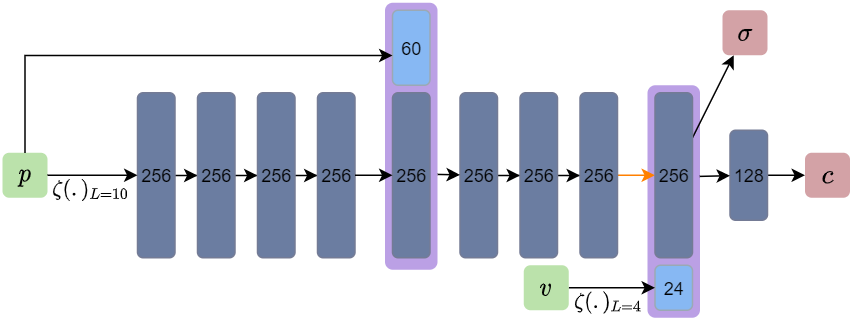
\includegraphics[width=0.6\textwidth]{img/mlp_nerf.png}
    \caption{MLP used in NeRF \cite{nerf2020mildenhall} Dark blue boxes represent hidden layers. Black arrows indicate FC-layers with sigmoid activation, orange arrows - FC-layers without activation. $\zeta(.)$ stays for positional encoding function. $\sigma$ is 1D volume density, $c$ is a 3D color value. }
    \label{fig:mlp_nerf}
\end{figure}

\cite{nrf2020} introduce neural reflectance field (NRF), which is a neural scene representation that implicitly encodes scene geometry (in form of volume density), normal and reflectance properties of the scene. Authors extend the idea of \cite{nerf2020mildenhall} by implying single-bounce single-point direct illumination from non-colocated light source by adding light transmittance term to the rendering equation. This requires using ray marching algorithm to light ray as well. Although the same technique of \textit{positional encoding} and \textit{hierarchical volume sampling} has been used, the rendering is still highly time inefficient, especially under novel non-colocated light and view. Even precomputing the light transmittance volume does not help much. Due to these performance difficulties authors only consider colocated light source in their experiments.

\cite{nsvf2020} try to alleviate this problem by introducing neural sparse voxel fields (NSVFs), which leverage the usage of sparse voxel octrees for scene representation. The usage of classical ray marching approach together with combination of implicit NeRFs and explicit octree structure results in more than 10 times faster renders comparing to \cite{nerf2020mildenhall}. Authors also use a bunch of techniques such as: \textit{self-prunning} of octrees and \textit{progressive training} for efficient handling essential and non-essential voxels. However, the light interaction is not modelled meaning that only global illumination is going to be implicitly represented in the model.

\cite{rebain2020derf} propose a framework to decompose the scene into multiple parts in order to increase the time efficiency of \cite{nerf2020mildenhall}'s approach. This implies parallel evaluation of the NeRF networks, which are responsible for different parts of the scene decomposed using Voronoi Diagrams \cite{aurenhammer1991voronoi} based method. The final image is composed using Painter's Algorithm \cite{Newell1972ANA}. This method does not model any light interaction thereby limiting scene reconstruction under novel light conditions.

\cite{boss2020nerd} follows the NeRF architecture, but introduce explicit decomposition and rendering steps. The authors use 2 networks: first for sampling points along the ray and the second one for estimating color and normal information as well as BRDF parameters of the scene, which implies physically plausible output values. The big advantage of this decomposition approach is a textured mesh extraction.

\cite{srinivasan2020nerv} extend the original NeRF approach not only for novel view but also for novel direct and indirect (one bounce) light conditions. The authors exploit a quite simple idea of predicting visibility and surface fields for the scene along with other appearance properties. These fields are used later for illumination estimation, which is plugged into rendering integral. Authors use 2 networks instead of one used in NeRF for predicting the volume density and appearance parameters. The normal map is calculated as negative gradient vector of the volume density predicted by MLP. Another (the 3rd) network learns to predict visibility and max. depth information, which allows to efficiently model the scene under one-bounce indirect illumination. The scheme of used MLPs is shown on \Cref{fig:mlp_nerv}

\begin{figure}[t]
    \centering
    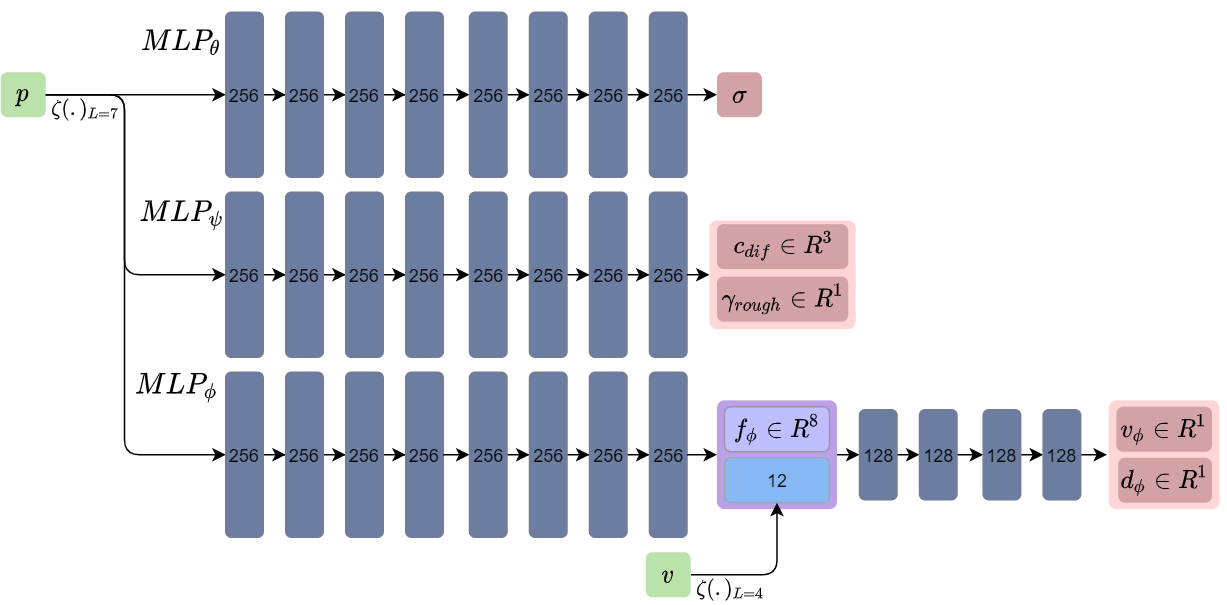
\includegraphics[width=0.6\textwidth]{img/mlp_nerv.png}
    \caption{Schematics for NeRD approach \cite{srinivasan2020nerv}. Two separate MLPs $MLP_\theta$ and $MLP_\psi$ are used to predict volume density $\sigma$ and appearance parameters diffuse albedo $c_{dif}$ as well as roughness $\gamma_{rough}$. The 3\textsuperscript{rd} MLP predicts visibility $v_\phi$ and max. depth $d_\phi$ values. Dark blue boxes represent hidden layers. Black arrows indicate FC-layers with ReLU activations.}
    \label{fig:mlp_nerv}
\end{figure}

A few recent works also focus on improving performance of such a group of approaches as 3D scene reconstruction. \cite{lindell2020autoint} employ neural networks for faster approximation of integral calculations in volume rendering tasks. \cite{tancik2020meta} improves the optimization trajectory of the model in coordinate-based neural representations such as NRF using so-called "Meta Initialization" instead of standard initialization of neural models.

\rphr{\cite{guo2020osf} so they adjust NeRF setup with 2 types of light-rays: intra-object (within the object) and inter-object (within the scene), right? and then they say, that intra-object light is modeled implicitly with MLP (light scattering), but inter-object light rays are traced explicitly (shadows casting). Does that mean, that they need semantic segmentation (to separate objects from the scene) for real-world cases? their results look quite appealing, and I like the idea of combining learnable and non-learnable light transport, but I don't see how this can work on real-world datasets (if I got their idea right)}

% \textbf{Metrics}


\section{Proposed Solution}

The proposed solution involves NRF as a scene representation together with the ray marching framework as proposed in \cite{nrf2020}. This allows not only to take into account view-dependant effects but also consider relighting re-rendered scene. In order to reduce the time consumption of the approach the effectiveness of sparse voxel octrees \cite{nsvf2020} can be leveraged. The extended NSVF architecture is then looks like as shown in \Cref{fig:mlp_nsvfnrf_explicit}


\begin{figure}[t]
    \centering
    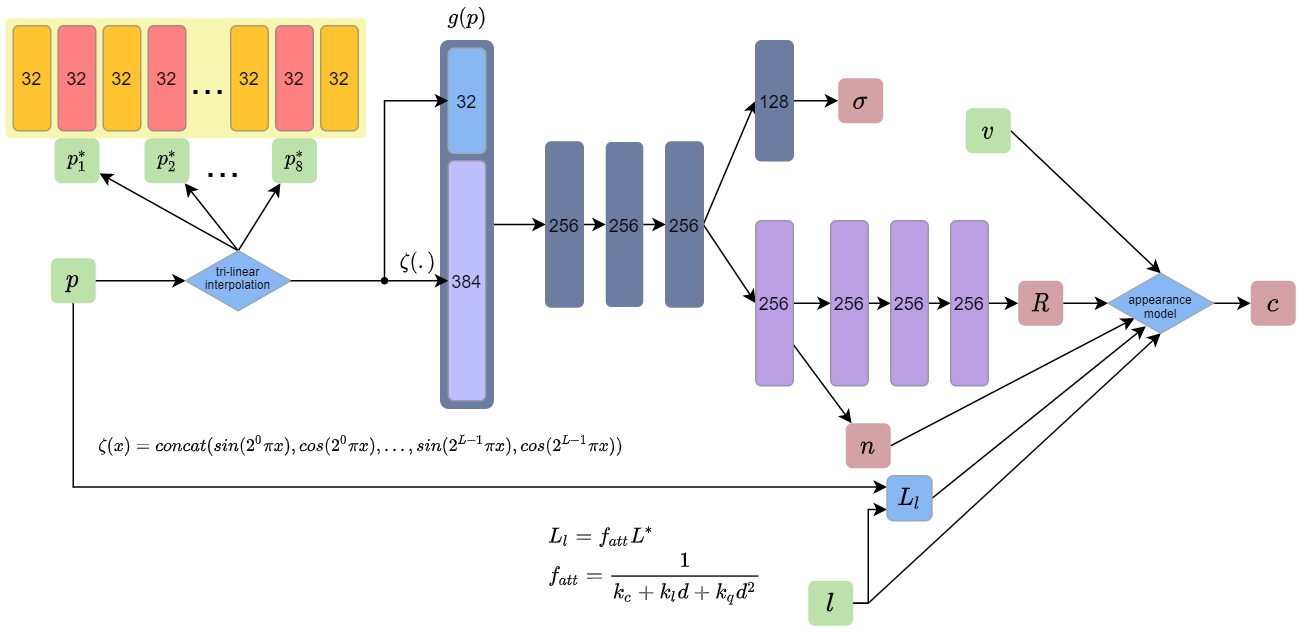
\includegraphics[width=0.6\textwidth]{img/mlp_nsvfnrf_explicit.png}
    \caption{The green boxes indicate inputs, the red boxes indicate outputs.
    % The left part of the scheme is responsible for encoding point in voxels' corners and then creating a Feature Field.
    Conceptually the architecture repeats the one proposed in \cite{nsvf2020}. However, instead of color the network outputs appearance vector $R$, which is then used (together with light and view directions, normal and light intensity) to evaluate appearance model. The $L_l$ denotes the light radiance considering the point light falloff.}
    \label{fig:mlp_nsvfnrf_explicit}
\end{figure}

% \begin{wrapfigure}{r}{0.4\textwidth}
%     \centering
%     \includegraphics[width=0.4\textwidth]{img/light_nrf.png}
%     \caption{}
%     \label{fig:mlp_nerf}
% \end{wrapfigure}


\begin{figure}[h]
    \centering
    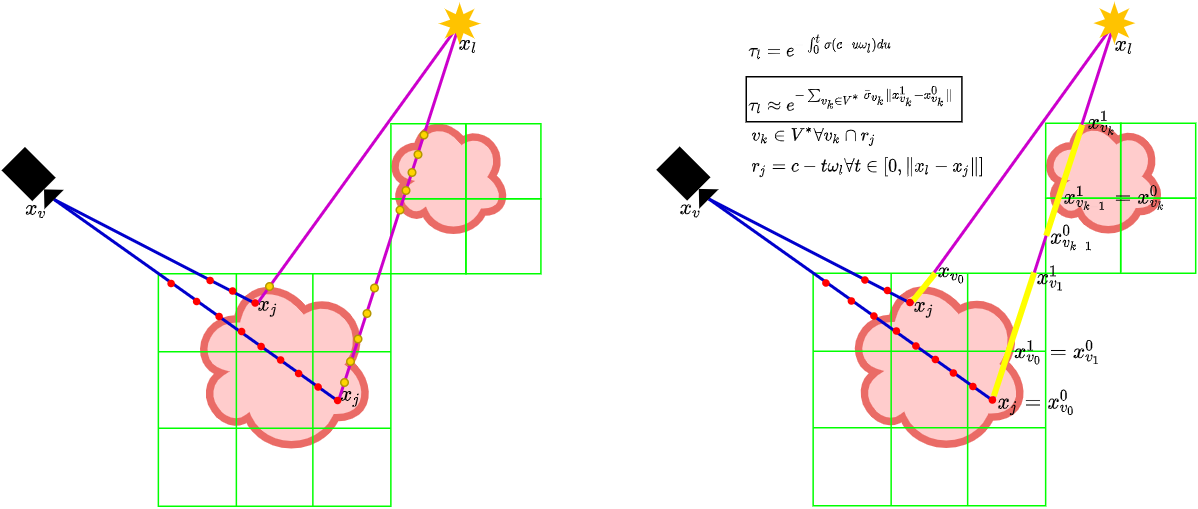
\includegraphics[width=0.75\textwidth]{img/light_nrf_approx_both.png}
    \caption{The sketch of how the view and light rays are sampled on the scene. The left part shows the same idea as used proposed by \cite{nrf2020} with the difference of using sparse voxel octree optimization (SVO), proposed by \cite{nsvf2020}. A lot of samples have to be sampled on light rays, which is very computationally demanding even with using SVO approach. The right part shows the proposed approximation for sampling the light rays. Assuming that the density inside each voxel is homogeneous, the collective transmittance of the voxels intersected by the ray is dependant on the distance the ray travelled inside the voxel. The transmittance decay outside the voxels is assumed negligible.}
    \label{fig:light_nrf_approx_both}
\end{figure}

Although this solution suppose to be more time effective, there is still a limitation for the colocated light source, because the light rays have to be sampled in a similar way the view rays are sampled (\Cref{fig:light_nrf_approx_both}, left). Assuming that the media inside the voxels is homogeneous this approach is going to be extended to non-colocated light sources by using approximation instead of real sampling for the light rays, as shown on \Cref{fig:light_nrf_approx_both} (right).


\begin{figure}[h]
    \centering
    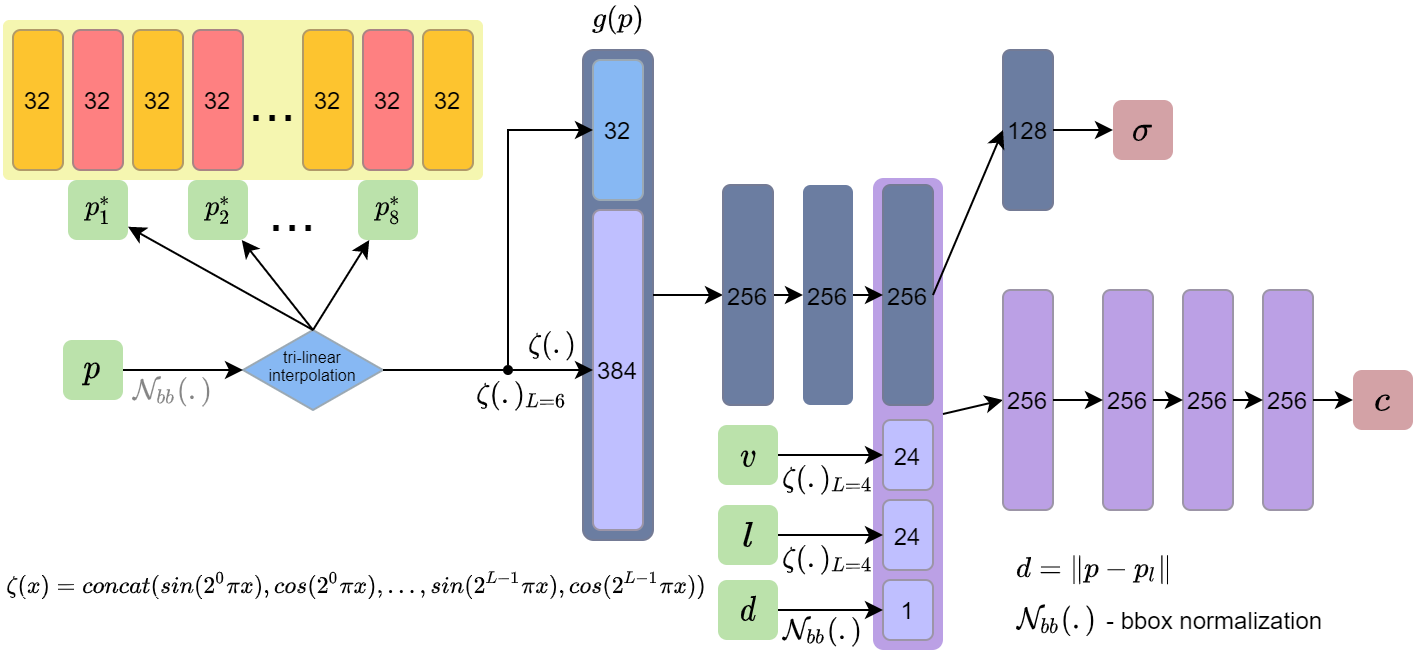
\includegraphics[width=0.75\textwidth]{img/mlp_nsvfnrf_implicit.png}
    \caption{The original NSVF (\cite{nsvf2020}) network is extended for modelling single point light illumination. The positionally encoded light direction $l$ is being concatenated with the distance to the point light source $d$, view direction $v$ and 3\textsuperscript{rd} hidden layer of denisity predictor to form a first layer of the Texture predictor that outputs color value $c$. Only 4 hidden layers of Texture predictor might not be enough and might have to be increased.}
    \label{fig:mlp_nsvfnrf_implicit}
\end{figure}

Originally the approach implies the usage of explicit reflectance model.
That means that the produced output is limited by used BRDF, e.g. the subsurface scattering effects are not modelled in BRDFs.
However, the implicit neural representation of reflectance model can remove these restrictions allowing to reproduce richer light- and view-dependant surface effects. The \Cref{fig:mlp_nsvfnrf_implicit} shows the network architecture based on NSVF approach (\cite{nsvf2020}), which is extended to model single point light illumination.

In original approach the input view direction is defined in global coordinate system.
In this case the MLP learns how the point looks like from the given view direction.
However, the appearance at the point is highly dependant on the normal of the surface.
That's why the network can be nudged to learn material appearance properties by using view and light directions transformed into local tangent frame.
The normal direction can be calculated using negative normalized gradient vector of the $\sigma$.

\rphr{Probably add here a few words on the BRDF that is going to be used (Cook-Torance -> Disnay ... vs. sggx}


\subsection{Road map}
\label{roadmap}

\begin{enumerate}

    \item \textit{Prepare synthetic dataset}
    The most of relevant works do not principally model light sources, which means that these datasets are not useful for the stated task.
    \cite{nrf2020} use datasets with colocated light, however authors did not expose any implementation as well as datasets from their work.
    \cite{srinivasan2020nerv} also use suitable synthetic datasets, but at the moment of writing they are not publicly available.
    This is the reason to create a synthetic dataset that contains the scene rendered from different viewpoints with colocated and non-colocated light sources.
    
    \item \textit{Sparse voxel octrees}
    Combine sparse voxel octrees optimization technique with the NRF. NSVF provide decent implementation which is going to be extended with appearance model from NRF. This also requires implementation of the proper rendering procedure.
    The model from \cite{nrf2020} outputs not color values but the reflectance parameters.
    This requires to apply the BRDF in order to get the color values of the rendering.
    
    \item \textit{Training/Evaluation stage}
    The training of the model is going to be done using prepared synthetic dataset consisting of samples with colocated light sources.
    \begin{itemize}
        \item The "test dataset" has to be chosen in a way it does not have any close-neighbour points, in order to test the model for generalization.
        \item The evaluation is to be compared with results of NRF-based approach \cite{nrf2020}
    \end{itemize}
    
    \item \textit{Neural reflectance model}
    Adjust the model such that it also implicitly represents the reflectance of the scene. This is going to be done by changing the structure of the neural reflectance field such that it outputs the color values instead of the reflectance parameters. This means that the reflectance model is implicitly modelled in the neural reflectance field. The model capacity might need to be adjusted in order to correspond to increased complexity of the model.
    
    \item \textit{Training/Evaluation stage}
    Repeat training with the neural reflectance representation.
    \begin{itemize}
        \item The evaluation involves comparison with base-line methods (more on that in \Cref{evaluation})
    \end{itemize}

    \item \textit{Non-colocated light extension}
    Extension for non-colocated light sources requires an approximation step in order to make the approach feasible.
    The offered technique is to approximate light transmittance only according to depth inside the sparse voxels instead of applying the whole ray marching framework for the light rays.
    \begin{itemize}
        \item \Cref{fig:light_nrf_approx_both} (right) shows formulas for calculating light transmittance inside voxels. The $\bar\sigma_{v_k}$ indicates an average transmittance inside the voxel. For efficiency purposes it has to be precomputed and recalculated throughout the training.
    \end{itemize}
    
    \item \textit{Training/Evaluation stage}
    Training the model on synthetic dataset with the non-colocated light sources.
    \begin{itemize}
        \item Compare results with the results from the previous step and with base-line methods as well
    \end{itemize}
    
    \item \textit{Real-world dataset}
    \cite{nrf2020} use some real-world scenes captured with a cell phone.
    Although this dataset contains only colocated light source (cell phone flashlight), it can still be used for training the model.
    Another source of real-world data can be captured with TAC7 scanning device \cite{tac7}, which uses sophisticated camera and light setup.
    \begin{itemize}
        \item Since TAC7 extracts the height map of the scene, it can be used for increasing performance of the method. Namely such technique as "self-pruning" for sparse voxel octrees is not needed anymore, because the information from the height map can be used to filter out empty voxels.
    \end{itemize}
    
    \item \textit{Training/Evaluation stage}
    Training and evaluation of the model on real-world dataset.
\end{enumerate}

\section{Evaluation}
\label{evaluation}

A vast majority of related works do not model light interaction, which makes them being as not good candidates to compare the results with.

\cite{nrf2020}'s approach is a basement of the proposed solution, therefore it is considered as a baseline method.

Although \cite{boss2020nerd} do not use light source in their setup, but they still extract complex appearance parameters, which makes the results to be comparable with those from the proposed solution.

\cite{srinivasan2020nerv} model both direct and indirect illumination and consequently use datasets captured with light positions. Since this work is one of the closest works to the proposed approach, it should definitely be compared qualitatively as well as quantitatively (evaluation timings) with the results to be obtained.

\section{Implementation details}

Implementation details of the proposed solution may undergo some changes during the working process, however the rough plan consists of the following:
\begin{itemize}
    \item \textit{Neural scene representation frameworks}
    \cite{nsvf2020} accompany their paper with the implementation, which is going to be used as a base implementation of the project and includes:
    \begin{itemize}
        \item Python3
        \item PyTorch (using Fairseq framework \cite{ott2019fairseq})
        \item CUDA
        \item Nvidia Apex library
    \end{itemize}
    
    \item \textit{Dataset-related tools}
    Tools:
    \begin{itemize}
        \item OpenGL-based rendering framework \cite{thies2019deferred} is going to be used for creating synthetic dataset
        \item Blender (alternative rendering option)
    \end{itemize}
    Datasets:
    \begin{itemize}
        \item Datasets captured by \cite{nrf2020} (when they will be available)
        \item TAC7 Appearance Scanner \cite{tac7} for capturing real-world dataset
    \end{itemize}
\end{itemize}

\section{Extension points}

Another way to increase the speed of the approach (2-3 times faster) is to decompose it into sub-scenes using Voronoi-based decomposition and employ multiple networks to these parts as proposed by \cite{rebain2020derf}. As soon as these implementations become available it can be plugged into the proposed method.

Auto integration technique from \cite{lindell2020autoint} has good prerequisites to be adopted to the proposed method and can also be used to make the method up to 10 times faster.

The proposed solution considers light ray to be represented the same way the view ray is represented using 3D vector. However, light ray can also be parametrized using half-vector, which allows to drop one dimension down assuming isotropic reflection of the scene. Experiments with this kind of parametrization are planned as an extension point of this work.

\section{Timeline}

\begin{figure}
\begin{chronology}[2]{0}{26}{\textwidth}
  \event[0]{2}{Prepare synthetic dataset}
  \event[2]{5}{Implement NSVF with appearance model}
  \event[5]{7}{Experiments with Neural reflectance model}
  \event[7]{10}{Non-colocated light extension}
  \event[10]{12}{\color{blue}Buffer}
  \event[12]{15}{Prepare real-world dataset}
  \event[15]{17}{Experiments with real-world data}
  \event[17]{19}{\color{blue}Buffer}
  \event[19]{26}{Writing thesis}
\end{chronology}
\caption{Timeline in weeks since the registration.}
\label{timeline}
\end{figure}

\Cref{timeline} sketches how I plan to use the 26 weeks from the registration of the thesis to its deadline.
The timeline echoes the road map described in \Cref{roadmap}.
It contains in addition two extra buffer periods, which are supposed to help me to stay on or ahead of the schedule in case of any unexpected complications.
The last weeks are reserved for writing the thesis text.
Note that this is only a rough plan on how the process is going to work out.
The phases are usually blending into each other.

\bibliographystyle{apalike} % We choose the "plain" reference style
\bibliography{refs} % Entries are in the "refs.bib" file

\end{document}
